\section{Occupation Number Formalism (Second Quantization)}
\subsection{Advantages of occupation number formalism}
Since simple things can sometimes get to look pretty formidable in second quantization it is a good idea to understand why many-body physicists all use it. \bluep{The first reason is that it enables us to deal with systems containing a \textbf{variable number of particles}}.It turns out to give an enormous flexibility in the formalism if \textbf{N is allowed to vary in intermediate stages of a calculation and becomes fixed only at the end.} For example, we can put in and remove test particles at will, as in the case of the propagator. Or we can introduce the particle-hole formalism in which the number of particles and holes is variable.

The second reason for the occupation number formalism has to do with the symmetry properties of Fermi and Boss system. Doing things the old
way, we always have to worry about the complicated business of keeping the wave function properly symmetrized. But it turns out that in second quantization, the \textbf{creation and destruction operators obey certain commutation rules which have built into them all the symmetry properties of the system}. By just using these rules we are automatically free from symmetrization headaches.

\subsection{Many-body wave function in occupation number formalism}
Imagine that we are given a system of N identical fermions, which are in general interacting with each other and with an external potential. We have seen that such a system may be described in terms of a set of basis states, $|n_1,...,n_l,...\rangle$ in which the $n_l$ meant $n_l$ particles in the unperturbed single-particle energy eigenstate, $\phi_l$. Actually, \redp{the single-particle states used can be any orthonormal set}. This means that in general, $|n_1,...,n_l,...\rangle$ are not energy eigenstates of either the interacting or the non-interacting system of particles and their choice is determined by convenience. Foe the moment, we will use the $\phi$'s which satisfy the Schrodinger equation:
\begin{equation}\begin{aligned}
H \phi_{k \sigma}(\mathbf{r}, \gamma) &=\epsilon_{k o} \phi_{k o}(\mathbf{r}, \gamma) \\
H=\frac{p^{2}}{2 m}+U(\mathbf{r}) &=-\frac{1}{2 m} \nabla^{2}+U(\mathbf{r}) \\
(\hbar&=1)
\end{aligned}\end{equation}
and $\gamma, \sigma$ are the spin co-ordinate and quantum number respectively. In the case $U(\mathbf{r})=0,$ this has the solutions:
\begin{equation}\begin{aligned}
\phi_{k \sigma}(\mathbf{r}, \gamma) &=\frac{1}{\sqrt{\Omega}} e^{+i \mathbf{k} \cdot \mathbf{r}} \eta_{\sigma}(\gamma) \\
\epsilon_{k} &=\frac{k^{2}}{2 m}(\hbar=1)
\end{aligned}\end{equation}
where $\eta$ is the spin eigenfunction. In general, $\sigma, \gamma$ will be suppressed for brevity, and $\mathbf{k}$ will be short for $\mathbf{k}, \sigma,$ and $\mathbf{r} \equiv \mathbf{r}, \gamma$. 

If there are now N identical non-interacting fermions, the Hamiltonian and Schrodinger equation become
\begin{equation}\begin{array}{c}
H_{0}=\sum_{l=1}^{N} H_{l}, \quad H_{0} \Phi\left(\mathrm{r}_{1}, \ldots, \mathrm{r}_{N}\right)=E \Phi\left(\mathrm{r}_{1}, \ldots, \mathrm{r}_{N}\right) \\
H_{i}=\frac{p^{2}}{2 m}+U\left(\mathrm{r}_{i}\right) ; \quad H_{i} \phi_{k_{i}}=\epsilon_{k_{i}} \phi_{k_{i}}
\end{array}\end{equation}
since the system consists of identical fermions, the wave function must be antisymmetric, i.e., change sign when any two particle co-ordinates are interchanged. This is accomplished by forming a $\Phi$ given by the Slater determinant.
\begin{equation}\Phi_{k_{1} \ldots \ldots k_{N}}\left(\mathrm{r}_{1}, \ldots, \mathrm{r}_{N}\right)=\frac{1}{(N !)^{\frac{1}{2}}} \sum_{P} \gamma_{P} P\left[\phi_{k_{1}}\left(\mathrm{r}_{1}\right) \phi_{k_{2}}\left(\mathrm{r}_{2}\right) \ldots \phi_{k_{N}}\left(\mathrm{r}_{N}\right)\right]\end{equation}
or
\begin{equation}\Phi_{k_{1}, \ldots, k_{N}}\left(\mathbf{r}_{1}, \ldots, \mathbf{r}_{N}\right)=\frac{1}{(N !)^{\frac{1}{2}}}\left|\begin{array}{c}
\phi_{k_{1}}\left(\mathbf{r}_{1}\right) \phi_{k_{1}}\left(\mathbf{r}_{2}\right) \ldots \phi_{k_{1}}\left(\mathbf{r}_{N}\right) \\
\vdots \\
\phi_{k_{N}}\left(\mathbf{r}_{1}\right) \phi_{k_{N}}\left(\mathbf{r}_{2}\right) \dots \phi_{k_{N}}\left(\mathbf{r}_{N}\right)
\end{array}\right|
\label{slater-determinant-2}
\end{equation}
In the first form, $P$ is the permutation operator which interchanges the $\mathbf{r}_{i}$ 's in all possible ways (starting from some standard order), and $\gamma_{P}=-1$ for an odd number of interchanges, and +1 for an even number. The fact that $\Phi=0$ when any two $k_{i}$ 's are equal means that there can't be more than one particle in any state.

A tricky thing about (\ref{slater-determinant-2}) is its sign. For example, in a two-particle system with one particle in state $\phi_{1}$, and the other in $\phi_3$, the wave function is $\Phi_{k_1=1,k_2=3}\equiv\Phi_{13}$ or $\Phi_{k_1=3,k_2=1}\equiv\Phi_{31}$. Since the particles are identical, these represent the same state, but by (\ref{slater-determinant-2}) they differ by a minus sign. To remove this ambiguity, we always write $\Phi$ with the $k$'s in standard order given by:
\begin{equation}\Phi_{k_{1}<k_{2}<\ldots<k_{N}}\end{equation}
A compact way of writing $\Phi$ is
\begin{equation}\begin{aligned}
\Phi_{k_{1}, k_{2}, \ldots, k_{N}}\left(\mathbf{r}_{1}, \mathbf{r}_{2}, \ldots, \mathbf{r}_{N}\right) &=\Phi_{n_{1}, \ldots, n_{i}, \ldots}\left(\mathbf{r}_{1}, \mathbf{r}_{2}, \ldots, \mathbf{r}_{N}\right) \\
&=\left\langle\mathbf{r}_{1}, \mathbf{r}_{2}, \dots, \mathbf{r}_{N} | n_{1}, \dots, n_{i}, \dots\right\rangle
\end{aligned}\end{equation}
It is important to remember that \redp{the $\left|n_{1}, \ldots, n_{1}, \ldots\right\rangle$ are orthogonal and normal because the $\Phi_{k_{1}, \ldots, k_{N}}$ are}, and we may write this in the various equivalent ways
\begin{equation}\begin{array}{l}
\begin{aligned}
&\left\langle n_{1}^{\prime}, n_{2}^{\prime}, \ldots, n_{1}^{\prime}, \ldots | n_{1}, n_{2}, \ldots, n_{1}, \ldots\right\rangle  \\
& \equiv\left(\Phi_{n_{1}^{\prime}, n_{2}^{\prime}\ldots, n_{l}^{\prime}, \ldots} , \Phi_{n_{1}, n_{2}, \ldots, n_{l}, \ldots}\right) \\
& \equiv \int d^{3} \mathbf{r}_{1} \ldots d^{3} \mathbf{r}_{N} \Phi_{n_{1}^{\prime}, n_{2}}^{\prime}, \ldots .\left(\mathbf{r}_{1}, \ldots, \mathbf{r}_{N}\right) \Phi_{n_{1}, n_{2}, \ldots}\left(\mathbf{r}_{1}, \ldots, \mathbf{r}_{N}\right) \\
&=\delta_{n_{1}^{\prime}, n_{1}} \delta_{n_{2}^{\prime}, n_{2}} \ldots \delta_{n_{l}^{\prime}, n_{l}} \cdots .
\end{aligned}
\end{array}\end{equation}
Now we take the step to allow $N$ to be variable, running from 0 to $\infty$. Thus generates the set of basis functions in the following table:
\begin{table}[H]
\caption{Complete set of basis functions used in second quantization}
\centering
\begin{tabular}{ccc}
\hline
N        & $\Phi_{k_1,k_2,...k_N}$                   & $=|n_1,n_2,\ldots,n_i,\ldots\rangle$                                     \\ \hline
0        & $\Phi_0$                                  & $|000\ldots\rangle$                                                      \\
1        & $\Phi_{1}, \Phi_{2}, \Phi_{3}, \ldots$    & $|100 \ldots\rangle,|0100 \ldots\rangle,|00100 \ldots\rangle \ldots$     \\
2        & $\Phi_{12}, \Phi_{13}, \Phi_{23}, \ldots$ & $|1100 \ldots\rangle,|101000 \ldots\rangle,|01100 \ldots\rangle, \ldots$ \\
$\vdots$ & $\vdots$                                  & $\vdots$                                                                
\end{tabular}
\end{table}
This Hilbert space may be pictured as follows:
\begin{equation}
    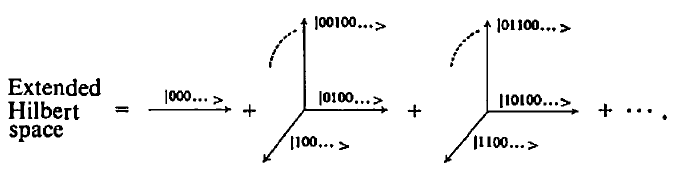
\includegraphics[width=0.8\textwidth]{screenshots/extended-hilbert-space.PNG}
\label{extended-hilbert-space}
\end{equation}

This set is often called 'occupation number basis', and the whole formalism is sometimes referred to as '\redp{occupation number representation}'. Note carefully that we did not get this new basis by unitary transformation (like, for example, is done in going from position to momentum basis).

Only systems of independent fermions without perturbing interactions of any sort have been considered thus far. In the presence of such interactions, \bluep{the $\left.| n_{1}, \ldots, n_{t}, \ldots\right)$ are no longer eigenstates of the total Hamiltonian for the system and the correct eigenstates must be obtained as the linear combination}
\begin{equation}\begin{aligned}
\Psi^{\prime} &=\Phi_{0}+\sum_{k_{1}} A_{k_{1}} \Phi_{k_{1}}+\sum_{k_{1}<k_{2}} A_{k_{1}, k_{2}} \Phi_{k_{1}, k_{2}}+\cdots \\
&=\sum_{n_{1}, \ldots, n_{i}, \ldots} A_{n_{1}, \ldots, n_{i}, \ldots}\left|n_{1}, \ldots, n_{i}, \ldots\right\rangle
\end{aligned}\end{equation}

\subsection{Operators in occupation number formalism}
It was pointed out in Chapter 4 that all operators in this new formalism may be expressed in terms of the creation and destruction operator $c_i^{\dagger}$,$c_i$. The definition of these operators must include a factor of $(\pm1)$ because of antisymmetry. Thus, if $c_i^{\dagger}$,$c_i$ act in such a sequence on the wave function that their net efferct is to exchange two particles, then the wave function must change its sign. Some thought shows that the proper definition is 
\begin{equation}\begin{array}{l}
c_{1}^{\dagger}\left|n_{1}, \ldots, n_{1}, \ldots\right\rangle=(-1)^{\Sigma_{i}}\left(1-n_{i}\right)\left|n_{1}, \ldots, n_{i}+1, \ldots\right\rangle \\
c_{1}\left|n_{1}, \ldots, n_{1}, \ldots\right\rangle=(-1)^{\Sigma_{i}} n_{i}\left|n_{1}, \ldots, n_{i}-1, \ldots\right\rangle
\end{array}\end{equation}
where $\Sigma_i=n_1+n_2+\ldots n_{i-1}$. That is, we get a factor of (-1) for each particle (i.e., each occupied state) standing to the left of the state i in the wave function.

One of the nice properties of the $c_{1}^{\dagger}$ operators is that by applying them repeatedly to the "true vacuum" state (state with no particles in it), it is possible to generate all other states, thus:
\begin{equation}\begin{array}{l}
\Phi_{k_{1}, k_{2}, \ldots, k_{N}}=c_{k_{1}}^{\dagger} c_{k_{2}}^{\dagger} \ldots c_{k_{n}}^{\dagger}|000 \ldots\rangle \\
\left|n_{1}, n_{2}, \ldots\right\rangle=\left(c_{1}\right)^{n_{1}}\left(c_{2}\right)^{n_{2}} \ldots|0000 \ldots\rangle
\end{array}\end{equation}
Another important property of the $c_{1}^{\dagger}, c_{l}$ operators is that they are \redp{\textbf{'hermitian adjoints'}} of each other. This can be seen by constructing matrices for them, using the $\left|n_{1} n_{2}, \ldots, n_{1}, \ldots\right\rangle$ 's as basis states
\begin{equation}
    \begin{aligned}
    &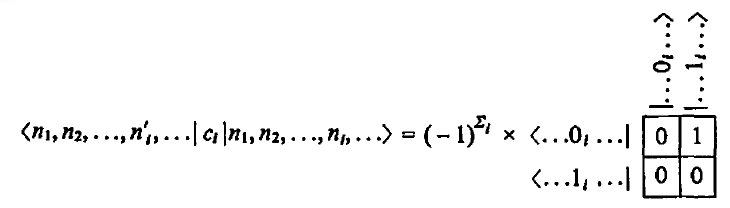
\includegraphics[width=0.8\textwidth]{screenshots/hermitian-adjoint-1.PNG}\\
    &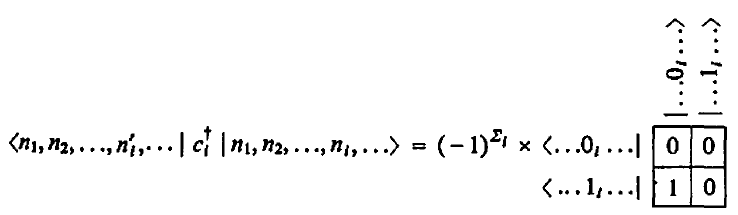
\includegraphics[width=0.8\textwidth]{screenshots/hermitian-adjoint-2.PNG}
    \end{aligned}
\end{equation}
so that
\begin{equation}c_{i}^{\dagger}=\left(c_{i}\right)^{\dagger}\end{equation}
\redp{\textbf{where $\dagger$ means hermitian adjoint. This further shows that $c_{h}^{\dagger} c_{l}$ are nonhermitian and are therefore not observables.}} (otherwise, we should have $c_i=c^{\dagger}_i$). Using the matrices above we can show that:
\begin{equation}\left(c_{i}^{\dagger} c_{i}\right)^{\dagger}=c_{i}^{\dagger} c_{i}\end{equation}
so that $c_i^{\dagger}c_i$ is hermitian. This combination is the famous "\textbf{\redp{number operator}}":
\begin{equation}\hat{n}_{l}=c_{l}^{\dagger} c_{l} ; \quad\left(\hat{N}=\sum_{l} c_{l}^{\dagger} c_{l}\right)\end{equation}
For example
$$c_{i}^{\dagger} c_{i}\left|n_{1}, \dots, n_{i}, \dots\right\rangle=n_{i}\left|n_{1}, \dots, n_{i}, \dots\right\rangle$$

\begin{imp}
The $c_{1}^{\dagger}, c_{1}$ operators obey the following important 'fermion commutation rules':
\begin{equation}
\begin{aligned}
&(1)\left[c_{l}, c_{k}^{\dagger}\right]_{+}=c_{l} c_{k}^{\dagger}+c_{k}^{\dagger} c_{l}=\delta_{l k}\\
&(2)\left[c_{l}, c_{k}\right]_{+}=0\\
&(3)\left[c_{l}^{\dagger}, c_{k}^{\dagger}\right]_{+}=0
\end{aligned}
\label{anti-cmmutation-rules-c}
\end{equation}
\end{imp}
These can be easily proved from the definitions:
$$\begin{aligned}
c_{1} c_{k}\left|n_{1}, \ldots, n_{1}, \ldots, n_{k}, \ldots\right\rangle &=(-1)^{\Sigma_{x}} n_{k} c_{l}\left|n_{1}, \ldots, n_{l}, \ldots, n_{k}-1, \ldots\right\rangle \\
&=(-1)^{\sum_{k}+\Sigma_{l}} n_{k} n_{l}\left|n_{1}, \ldots, n_{l}-1, \ldots, n_{k}-1, \ldots\right\rangle
\end{aligned}$$
$$\begin{aligned}
c_{k} c_{l}\left|n_{1}, \ldots, n_{l}, \ldots, n_{k}, \ldots\right\rangle &=(-1)^{\Sigma_{l}} n_{l} c_{k}\left|n_{1}, \ldots, n_{l}-1, \ldots, n_{k}, \ldots\right\rangle \\
&=(-1)(-1)^{\Sigma_{k}+\Sigma_{l}} n_{k} n_{l}\left|n_{1}, \ldots, n_{l}-1, \ldots, n_{k}-1, \ldots\right\rangle
\end{aligned}$$
where the extra (-1) on line four comes from the fact that there is one less particle to the left of state k. Adding the two equations yields the second rule in (\ref{anti-cmmutation-rules-c}).

The importance of the above sets of' anti-commutation' relations lies in the fact that all the antisymmetry properties are built into them. Therefore, by using them in the right places, we don't have to worry either about the symmetry of the wave functions themselves.

\textbf{\redp{Let us now consider how to express the usual quantum operators in terms of $c_i^{\dagger}$,$c_i$.}} \textbf{We require equality between the matrix elements of the operator as computed in occupation number formalism and in the old cave-man formalism. For example, in a one-particle system, the operator $\mathcal{O}(\mathbf{r,p})$ with matrix elements:}
\begin{equation}O_{ij}=\left\langle\phi_{1}|\mathcal{O}| \phi_{j}\right\rangle=\int \phi_{i}^{*}(\mathbf{r}) \mathcal{O}(\mathbf{r}, \mathbf{p}) \phi_{j}(\mathbf{r}) d^{3} \mathbf{r}\end{equation}
has the occupation number form
\begin{equation}\mathcal{O}^{\mathrm{occ}}=\sum_{\boldsymbol{k}, l} \mathcal{O}_{k l} c_{k}^{\dagger} c_{l}\end{equation}
This is easily checked as
\begin{equation}\begin{aligned}
\left\langle 00 \ldots 1_{i} \ldots\left|\theta^{occ}\right| 00 \ldots 1_{j} \ldots\right\rangle &=\sum_{k, l} \mathcal{O}_{k l}\left\langle 00 \ldots 1_{i} \ldots\left|c_{k}^{\dagger} c_{l}\right| 00 \ldots 1_{j} \ldots\right\rangle \\
&=\sum_{k, l} \mathcal{O}_{k l} \delta_{lj} \delta_{i k}\\
&=\mathcal{O}_{ij}
\end{aligned}\end{equation}
Suppose we have an operator
\begin{equation}\mathcal{O}=\sum_{i=1}^{N} \mathcal{O}\left(\mathbf{r}_{i}, \mathbf{p}_{i}\right)\end{equation}
like for example the external potential:
\begin{equation}V\left(\mathbf{r}_{1}, \dots, \mathbf{r}_{N}\right)=\sum_{i=1}^{N} V\left(\mathbf{r}_{i}\right)\end{equation}
Such operators are called \redp{"one-body"} operators sicne they are a sum of operators each of which acts separately on one particle. Thus we have the valuable result that \textbf{\redp{in occupation number formalism, the single-particle operators have a form independent of N.}}

In a similar way, it can be shown that the "two-body" operator
\begin{equation}\mathcal{O}=\frac{1}{2} \sum_{\substack{i, j=1\\(i \neq j)}}^{N} \mathcal{O}\left(\mathbf{r}_{l}, \mathbf{p}_{i}, \mathbf{r}_{j}, \mathbf{p}_{j}\right)\end{equation}
For instance the interaction potential
\begin{equation}V\left(\mathbf{r}_{1}, \dots, \mathbf{r}_{N}\right)=\frac{1}{2} \sum_{\substack{i, j=1\\ (i \neq j)}} V\left(\mathbf{r}_{i}-\mathbf{r}_{j}\right)\end{equation}
becomes
\begin{equation}\mathcal{O}^{\mathrm{occ}}=\frac{1}{2} \sum_{k l m n} \mathcal{O}_{k \operatorname{lm} n} c_{l}^{\dagger} c_{k}^{\dagger} c_{m} c_{n}\end{equation}
where
\begin{equation}\mathcal{O}_{klmn}=\int d^{3} \mathbf{r} \int d^{3} \mathbf{r}^{\prime} \phi_{k}^{*}(\mathbf{r}) \phi_{i}^{*}\left(\mathbf{r}^{\prime}\right) \mathcal{O}\left(\mathbf{r}, \mathbf{r}^{\prime} ; \mathbf{p}, \mathbf{p}^{\prime}\right) \phi_{m}(\mathbf{r}) \phi_{n}\left(\mathbf{r}^{\prime}\right)\end{equation}
We remark here that the results also hold true in the case of bosons.\textbf{If by now you are still confused by the subscript sequence in $c_l^{\dagger}c_k^{\dagger}c_mc_n$, please check Appendix A.}

\subsection{Hamiltonian and Schrodinger equation In occupation number formalism}